
    \section*{CS6000 - Computer Science Research - Git Assignment}
    By Duane Michael
    
    \today
 

\begin{figure}[h]
    \centering
    \fbox{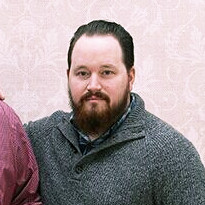
\includegraphics{Michael_Headshot.jpg}}
    \caption{A photo of Duane Michael}
    \label{fig:headshot}
\end{figure}
I am a first year PhD student in the computer science program. Professionally, I work in computer security specializing in offensive security, such as penetration testing, exploit development, vulnerability research, etc. My current academic research interests relate to the application of machine learning and artificial intelligence techniques, such as artificial neural networks and deep learning, to detect intrusions and anomalous behavior on a network or system. I am also interested in various other areas of computer security, so I am expecting my research interests to shift until I get settled into the program.

\testbf{Question from IJ Olawale}
Hello Michael, thank you for sharing your professional and research interests. With your decision to start a PhD program, do you see yourself transiting from your professional career to the academia? For me, I have worked in the corporate world since I graduated from college, over 20 years ago and now it is a bit of struggle getting back into the world of reading voluminous testbooks, research papers, assignments and exams! LOL... Wishing you the best in your PhD pursuit.
\\

\textbf{Answer to IJ Olawale}
Hi IJ, This is a great question and something I have thought about in depth. I can definitely see myself going towards academia at some point. My priority is advancing the state of security, and I believe there is important work to be done both in academia and industry. Getting into the swing of graduate school has been quite a whirlwind! My first few weeks of my algorithms class were pretty intense for me, but I feel like I'm finally finding my stride!
